În tabelul de mai jos se prezintă o analiză comparativă între rezultatele obținute în urma rulării proprii și cele obținute în cadrul competiției. Fișierele cu rezultatele rulărilor pot fi accesate la următoarele linkuri:
\href{https://docs.google.com/spreadsheets/d/1iGJHwePCzW0axJIwVes_eiN3R4ppvNu-ndrO_Fy5dL0/edit#gid=1265769327}{rezultate competiție }
\href{https://docs.google.com/spreadsheets/d/1kSxunni8qgQLT6ZkCRWvSO2VMy2Hz7qA/edit#gid=1476783028}{rezultate echipă}

\begin{figure}[h]
\centering 
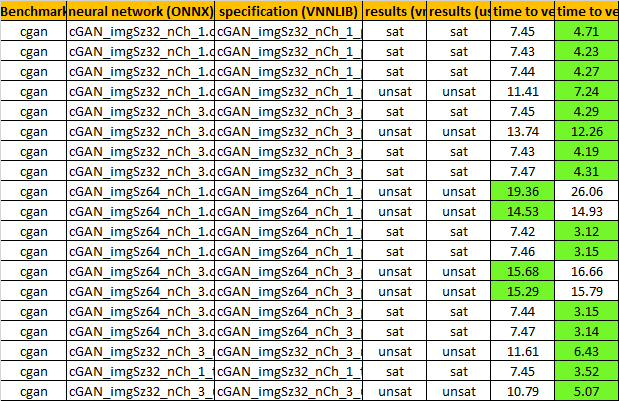
\includegraphics[width=0.8\linewidth]{imagini/interpretare rezultate/abC_comp_vs_us.png}
\caption{Rezultate alpha-beta-CROWN}
\label{fig:image1} 
\end{figure}

Din tabelul \ref{fig:image1}, este de notat faptul că pentru fiecare intrare, rezultatele(sat/unsat) au fost aceleași, atât pentru rezultatele rulării noastre, cât și pentru cele din competiție. Diferenta dintre competitie si echipa o constituie timpul de verificare. Timpul de verificare înregistrat al echipei este mai mic cu aproximativ 3 secunde pentru intrările unde rezultatul este satisfiabil. În schimb, pentru intrările cu rezultat nesatisfiabil timpul de verificare este considerabil mai mare.

Conform tabelului prezentat în \ref{fig:image1}, este de remarcat faptul că pentru fiecare intrare, rezultatele satisfiabil/nesatisfiabil) au fost aceleași, atât pentru rezultatele rulării proprii, cât și pentru cele din competiție. Diferența majoră între competiție și echipa noastră o constituie timpul de verificare. Timpul de verificare înregistrat al echipei noastre este mai mic cu aproximativ 3 secunde pentru intrările cu rezultat satisfiabil. În schimb, pentru intrările cu rezultat nesatisfiabil, timpul de verificare este considerabil mai mare.